\documentclass[nobib]{tufte-handout}

%\\geometry{showframe}% for debugging purposes -- displays the margins

\newcommand{\bra}[1]{\left(#1\right)}
\usepackage{amssymb}
\usepackage{hyperref}
\usepackage{pgfplots}
\usepackage[activate={true,nocompatibility},final,tracking=true,kerning=true,spacing=true,factor=1100,stretch=10,shrink=10]{microtype}
\usepackage{color}
\usepackage{steinmetz}
\usepackage{placeins}
\usepackage{adjustbox}
% Fixes captions and images being cut off
\usepackage{marginfix}
\usepackage{array}
\usepackage{tikz}
\usepackage{amsmath,amsthm}
\usetikzlibrary{shapes}
\usetikzlibrary{positioning}
\usepackage{listings}
\usepackage{forest}
\usepackage{colortbl}
\usepackage{caption}
\DeclareCaptionFont{white}{\color{white}}
\DeclareCaptionFormat{listing}{\colorbox{gray}{\parbox{\textwidth}{#1#2#3}}}
\captionsetup[lstlisting]{format=listing,labelfont=white,textfont=white}

% Set up the images/graphics package
\usepackage{graphicx}
\setkeys{Gin}{width=\linewidth,totalheight=\textheight,keepaspectratio}
\graphicspath{{.}}

\title{Notes for ECE 36800 - Data Structures and Algorithms}
\author[Shubham Saluja Kumar Agarwal]{Shubham Saluja Kumar Agarwal}
\date{\today}  % if the \date{} command is left out, the current date will be used

% The following package makes prettier tables.  We're all about the bling!
\usepackage{booktabs}

% The units package provides nice, non-stacked fractions and better spacing
% for units.
\usepackage{units}

% The fancyvrb package lets us customize the formatting of verbatim
% environments.  We use a slightly smaller font.
\usepackage{fancyvrb}
\fvset{fontsize=\normalsize}

% Small sections of multiple columns
\usepackage{multicol}

% For finite state machines 
\usetikzlibrary{automata} % Import library for drawing automata
\usetikzlibrary{positioning} % ...positioning nodes
\usetikzlibrary{arrows} % ...customizing arrows
\tikzset{node distance=2.5cm, % Minimum distance between two nodes. Change if necessary.
    every state/.style={ % Sets the properties for each state
    semithick,
    fill=gray!10},
    initial text={}, % No label on start arrow
    double distance=2pt, % Adjust appearance of accept states
    every edge/.style={ % Sets the properties for each transition
    draw,
    ->,>=stealth', % Makes edges directed with bold arrowheads
    auto,
    semithick}}
\let\epsilon\varepsilon

% These commands are used to pretty-print LaTeX commands
\newcommand{\doccmd}[1]{\texttt{\textbackslash#1}}% command name -- adds backslash automatically
\newcommand{\docopt}[1]{\ensuremath{\langle}\textrm{\textit{#1}}\ensuremath{\rangle}}% optional command argument
\newcommand{\docarg}[1]{\textrm{\textit{#1}}}% (required) command argument
\newenvironment{docspec}{\begin{quote}\noindent}{\end{quote}}% command specification environment
\newcommand{\docenv}[1]{\textsf{#1}}% environment name
\newcommand{\docpkg}[1]{\texttt{#1}}% package name
\newcommand{\doccls}[1]{\texttt{#1}}% document class name
\newcommand{\docclsopt}[1]{\texttt{#1}}% document class option name

% Define a custom command for definitions and biconditional
\newcommand{\defn}[2]{\noindent\textbf{#1}:\ #2}
\let\biconditional\leftrightarrow

\begin{document}

\maketitle

\begin{abstract}
    These are lecture notes for spring 2024 ECE 36800 at Purdue. Modify, use, and distribute as you please.
\end{abstract}

\tableofcontents

\section{Course Introduction}
Provides insight into the use of data structures. Topics include stacks, queues
and lists, trees, graphs, sorting, searching, and hashing. The learning
outcomes are:
\begin{itemize}
    \item Advanced programming ideas, in practice and in theory
    \item Data structures and their abstractions: Stacks, lists, trees, and graphs
    \item Fundamentals of algorithms and their complexities: Sorting, searching, hashing,
          and graph algorithms
    \item Problem-Solving
\end{itemize}
\pagebreak

\section{Introduction to Data Structures \& Algorithms}
Data Structures are methods of organizing information for ease of manipulation.
Examples:
\begin{enumerate}
    \item Dictionary
    \item Check-out line or queues
    \item Spring-loaded plate dispenser or stacked
    \item Organizational Chart or tree
\end{enumerate}
These are associated with methods known as algorithms to be manipulated\\
Algorithms are methods of doing something.
Examples:
\begin{enumerate}
    \item Multiplying two numbers
    \item Making a sandwich
    \item Getting dressed
\end{enumerate}
The topics of interest within them are:\\
\begin{itemize}
    \item Correctness
    \item Efficiency in time and space
\end{itemize}
\section{Time Complexity Analysis}
The questions to be asked about an algorithm are the following:
\begin{itemize}
    \item Is it correct?
    \item Is it as fast as possible?
    \item How many machine instructions (in terms of n) does it take?
\end{itemize}
Let us take the following algorithm to add the numbers form 1 to n:
\begin{lstlisting}
    total = 0;
    for (i=1:n)
        total = total + i;
    return total
\end{lstlisting}
The cost will be:\\
\begin{table}
    \centering
    \begin{tabular}{c|c|c}
        Cost  & Frequency & Function                     \\
        \hline
        $C_1$ & 1         & Assign initial value         \\
        $C_2$ & n+1       & For loop iterations and exit \\
        $C_3$ & n         & Number additions             \\
        $C_4$ & 1         & Return value                 \\
    \end{tabular}
\end{table}
\FloatBarrier
The total is then:\\
\begin{align*}
    C_1*1+C_2(n+1)+C_3(n)+C_4(1) & = (C_2+C_3)n+ (C_1+C_2)+C_4
\end{align*}
However the $O(n)$ will only be n, as the constants and coefficients of these will be deprecated, as we will come to understand in more detail as this topic continues.\\
Let us take another example of some code that has a
\begin{align*}
    T(n)                                     & = n^2 + 10^7n+10^{10}                                \\
    T(10^{11})                               & = 10^{22} + 10^{18}+ 10^{10}                         \\
    T(2*10^{11})                             & = 4*10^{22} + 2*10^{18}+ 10^{10}                     \\
    \implies \frac{T(2*10^{11})}{T(10^{11})} & \approx 4 = \left(\frac{2*10^{11}}{10^{11}}\right)^2
\end{align*}
This goes to show that this algorithm has an $O(n) = n^2$, and all coefficients and lower order terms that are a part of the complexity are largely irrelevant for large n values.
This is why this is called \textbf{asymptotic notation}.\\
Another example of a simple algorithm is
\begin{lstlisting}
    total = 0;
    for (i=1:n):
        if (((i*i%3)==0)||((i*i%7)==0)):
            total = total+i*i;
    return total;
\end{lstlisting}
Which has a cost table that looks like the following:\\
\begin{table}
    \centering
    \begin{tabular}{c|c|c}
        Cost  & Frequency                                                                                  & Function                     \\
        \hline
        $C_1$ & 1                                                                                          & Assign initial value         \\
        $C_2$ & n+1                                                                                        & For loop iterations and exit \\
        $C_3$ & n                                                                                          & Number of $i\%3$ comparisons \\
        $C_4$ & $n - \lfloor \frac{n}{3} \rfloor  $                                                        & Number of $i\%7$ comparisons \\
        $C_5$ & $\lfloor \frac{n}{3} \rfloor + \lfloor \frac{n}{7} \rfloor - \lfloor \frac{n}{21} \rfloor$ & Number of additions          \\
        $C_6$ & 1                                                                                          & Returning value              \\
    \end{tabular}
\end{table}
It can be noted that $O(n) = n$ for this function, despite all the other complexities in the algorithm. However, it is important to know how to calculate $T(n)$ as well.\\
Now, let us look at something more complicated, matrix multiplication of two lower triangular matrices.
\begin{lstlisting}
    for (i=1:n):
        for (j=1:i):
            C_ij = 0;
            for (k=j:i):
                C_ij = C_ij+A_ik*B_kj
    return C
\end{lstlisting}
This has a cost table that looks like the following:
\begin{table}
    \centering
    \begin{tabular}{c|c|c}
        Cost  & Frequency                                        & Function                    \\
        \hline
        $C_1$ & n+1                                              & First loop                  \\
        $C_2$ & $\sum_{i=1}^{n} (i+1)$                           & Second loop                 \\
        $C_3$ & $\sum_{i=1}^{n} \sum_{j=1}^{i} 1 $               & Number of assigns           \\
        $C_4$ & $\sum_{i=1}^{n} \sum_{j=1}^{i} (i-j+2) $         & Third loop                  \\
        $C_5$ & $\sum_{i=1}^{n} \sum_{j=1}^{i} \sum_{k=j}^{i} 1$ & Number of assigns to matrix \\
        $C_6$ & 1                                                & Returning value             \\
    \end{tabular}
\end{table}
Finally, we can analyze an example that has logarithmic complexities.
\begin{lstlisting}
    i=2;
    k=0;
    while (i<n){
        i=i*i;
        k=k+1;
    }
    return i;
\end{lstlisting}
Which has a cost table that looks like the following:\\
\begin{table}
    \centering
    \begin{tabular}{c|c|c}
        Cost  & Frequency                          & Function                        \\
        \hline
        $C_1$ & 1                                  & Assign i                        \\
        $C_2$ & 1                                  & Assign k                        \\
        $C_3$ & $\lceil \log_2(\log_2(n))\rceil+1$ & Number of while loop iterations \\
        $C_4$ & $\lceil \log_2(\log_2(n))\rceil $  & number of assigns of i          \\
        $C_5$ & $\lceil \log_2(\log_2(n))\rceil$   & Number of k assigns             \\
        $C_6$ & 1                                  & Returning value                 \\
    \end{tabular}
\end{table}

It can be noted that if line three was instead changed to\\
\begin{lstlisting}
    while (i<=n){
\end{lstlisting}
The table will instead be:\\
\begin{table}
    \centering
    \begin{tabular}{c|c|c}
        Cost  & Frequency                            & Function                        \\
        \hline
        $C_1$ & 1                                    & Assign i                        \\
        $C_2$ & 1                                    & Assign k                        \\
        $C_3$ & $\lceil \log_2(\log_2(n+1))\rceil+1$ & Number of while loop iterations \\
        $C_4$ & $\lceil \log_2(\log_2(n+1))\rceil $  & number of assigns of i          \\
        $C_5$ & $\lceil \log_2(\log_2(n+1))\rceil$   & Number of k assigns             \\
        $C_6$ & 1                                    & Returning value                 \\
    \end{tabular}
\end{table}
\FloatBarrier
As the loop break condition changed from $i\geq n$ to $i\geq n+1$ by simply changing.
\section{Insertion and Shell Sort}
Sorting is necessary to process items in sorted order. It speeds up the
location of items, finding identical items, etc. \\ It is good to know that in
real life, what is sorted is in fact the pointers of these structs, as the
movement of structs have higher memory requirements.
\subsection{Insertion Sort}
Inserts an item into a sorted array. Compares the item with items in the sorted
array, and if they are in the incorrect order, they are swapped. This is
continued until everything has been successfully sorted.\\ The code to sort $n$
integers in an array $r$ looks like this:
\begin{lstlisting}
    for (j=1:n-1){
        for (i=j:1){
            if (r[i-1]>r[i]){
                swap(r[i-1], r[i]);
            }
            else{
                break;
            }
        }
    }
\end{lstlisting}
This is suboptimally inefficient due to the restriction of only swapping with
neighbors, directly. However, it can be made even more efficient using the
following algorithm:
\begin{lstlisting}
    for (j=1:n-1){
        temp = r[j];
        for (i=j:1){
            if (r[i-1]>temp_r){
                r[i] = r[i-1];
            }
            else{
                break;
            }
        }
        r[i] = temp_r;
    }
\end{lstlisting}
This allows us to "move" items down without constant comparisons, saving us
some assignments.\\ This can also be implemented using while loops, and thus
avoiding break:
\begin{lstlisting}
    for (j=1:n-1){
        temp=r[j];
        i=j;
        while (i>0 and r[i-1]>temp){
            r[i] = r[i-1];
            i-=1;
        }
        r[i]=temp_r;
    }
\end{lstlisting}
This has the following cost table in the best case:
\begin{table}
    \centering
    \begin{tabular}{c|c|c}
        Cost  & Frequency & Function                         \\
        \hline
        $C_1$ & n         & For loop iterations              \\
        $C_2$ & n-1       & Assign temp                      \\
        $C_3$ & n-1       & Assign i                         \\
        $C_4$ & n-1       & It is checked once per iteration \\
        $C_5$ & 0         & Number of r[i] exchanges         \\
        $C_6$ & 0         & Number of decreases  of i        \\
        $C_7$ & n-1       & Assign r[i]                      \\
    \end{tabular}
\end{table}
Which has a complexity $O(n)=n$
And the following in the worst case:
\begin{table}
    \centering
    \begin{tabular}{c|c|c}
        Cost  & Frequency              & Function                                 \\
        \hline
        $C_1$ & n                      & For loop iterations                      \\
        $C_2$ & n-1                    & Assign temp                              \\
        $C_3$ & n-1                    & Assign i                                 \\
        $C_4$ & $\frac{(n+2)(n-1)}{2}$ & Number of time the while loop is checked \\
        $C_5$ & $\frac{(n)(n-1)}{2}$   & Number of r[i] exchanges                 \\
        $C_6$ & $\frac{(n)(n-1)}{2}$   & Number of decreases of i                 \\
        $C_7$ & n-1                    & Assign r[i]                              \\
    \end{tabular}
\end{table}
Now, we will learn how to calculate the average performance of an algorithm like insertion sort.\\
Let us take a random $j^{th}$ item. The probability of it not needing to be moved is $\frac{1}{j+1}$. And it will need a certain some number between 0 and j exchanges to get to its rightful position if not.
This leads the expected total number of exchanges to be $\sum_{i=0}^j\frac{i}{j+1} = \frac{j}{2}$. Once we reach the $(n-1)^{th}$ element, this is $\frac{1}{2}\frac{n(n-1)}{2}\approx\frac{n^2}{4}$.\\ Average performance is seldom calculated for the intents and purposes of this course.\\
There are still some inefficiencies in insertion sort that can be improved by using sentinels.
\begin{lstlisting}
    for (j=n-1:1){
        if (r[j]<r[j-1]){
            swap(r[j], r[j-1]);
        }
    }
    for (j=2:n-1){
        temp=r[j];
        i=j;
        while (r[i-1]>temp){
            r[i] = r[i-1];
            i-=1;
        }
        r[i]=temp_r;
    }
\end{lstlisting}
By moving the smallest item to the beginning, we can avoid the (i>0) condition,
slightly increasing efficiency.\\
\subsection{Shell Sort}
This improves insertion sort by allowing for swaps along larger distances
between elements.\\ If we did 7-sorting and 3-sorting:\\ We would start with 7
subarrays with at most $\lceil \frac{n}{7} \rceil$ elements. These subarrays
would need to be sorted within themselves.\\ We would then go over to having 3
subarrays with at most $\lceil \frac{n}{3} \rceil$ elements. These subarrays
would once again need to be sorted within themselves.\\ Finally, we would
conduct regular insertion sort. The complexity of shell sort changes based on
the selected sequence.\\
\begin{itemize}
    \item $1,3,7,15, \ldots, 2^k-1, \ldots$ has a complexity of $O(n^{1.5})$
    \item $1,4,13,\ldots, 3h(k-1), \ldots$ also has a complexity of $O(n^{1.5})$
    \item $2^p3^q$ has a complexity $O(n(\log(n))^2)$
\end{itemize}
The algorithm of shell sort is the following:
\begin{lstlisting}
    for (j=k:n-1){
        temp=r[j];
        i=j;
        while (i>=k and r[i-k]>temp){
            r[i]=r[i-k];
            i=i-k;
        }
        r[i]=temp;
    }
\end{lstlisting}
To prove the complexity of the $2^p3^q$ complexity, we can visualize the
following triangle:
\begin{align*}
     & 1             \\
     & 2\;3          \\
     & 4\;6\;\;9     \\
     & 8\;12\;18\;27 \\
\end{align*}
which holds the values of k from the above algorithm the height and base of the triangle both have complexities of $\log(n)$, while the sorting of the subset make by each k has a complexity of $n$, which results in a total complexity of $n(\log(n))^2$.\\
Let us consider a triangle of the following form:
\begin{align*}
     & a      \\
     & 2a\;3a \\
\end{align*}
If one were to start with the largest and go to the smallest, that is, if one were to $3a$-sort, and then $2a$-sort, all numbers in the array would be at most $a$ positions away from their correct positions.\\
This can be semi-trivially proven under the assumption that if an array is $3a$-sorted and then $2a$-sorted, it will still be $3a$-sorted. This will not be solved in this document as it is a homework assignment.\\
\section{Asymptotic Notation}
The number of instructions executed is dependent on the number of inputs. As it
gets larger, the number of instructions increases too.\\ This has been
generalized and classified using asymptotic notation.
\begin{equation*}
    f(n) = O(g(n)) \iff \exists (c,n_0) \text{ such that }f(n)\leq cg(n) \quad \forall (n \geq n_0)
\end{equation*}
\textit{Note :If the space complexity is $O(g)$, the time complexity will be at least $O(g)$.\\}
The graphical representation of the above definition $O(n)$ is :
\begin{center}
    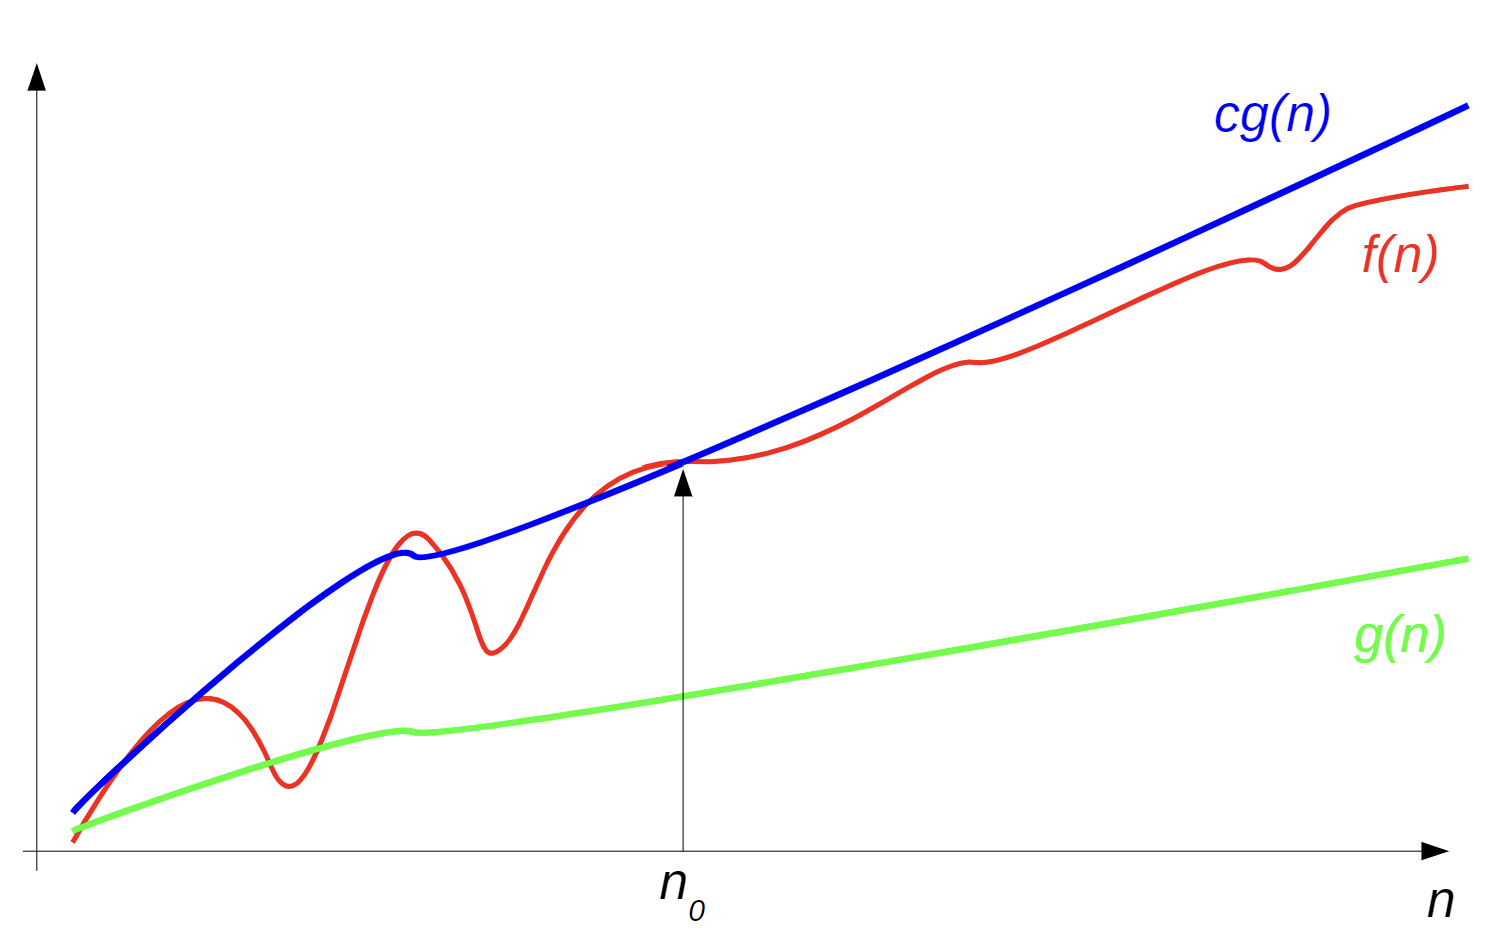
\includegraphics[width = 200px]{images/complexity_graph.png}
\end{center}
The values of $c$ and $n_0$ can be variable, and have any value, as long as the condition is fulfilled.\\
However, we are searching for $g(n)$ such that it refers to the smallest and simplest possible function of $n$ to allow for the existence of the values of $c$ and $n_0$ that will make the condition true.\\
A good strategy to select $c$ is the sum of the absolute values of all the coefficients in $f(n)$.\\
\textit{Note: $f(n)$ is equivalent to the $T(n)$ in the Time Complexity Analysis section.}\\
Another proof of $f(n)=O(g(n))$ is $\lim_{n \rightarrow \infty}\frac{f(n)}{g(n)}\neq \infty$.\\
However, it is not really necessary to go to this extent to find $c$ as there are several easier ways to find valid values. This method is an unnecessary complication for most cases.\\
For $g(n)$ to be useful, it should be simpler than $f(n)$ such as $1,n,n^2$, $n\log(n), 2^n, n!$.\\
However, once we go to exponential functions or above, the algorithms cease to be useful.\\
Some properties of asymptotic notation are:
\begin{align*}
    f(n)                  & =O(f(n))                                                            \\
    f(n)=O(g(n))\quad     & \& \quad g(n) = O(h(n)) \implies f(n)=O(h(n))                       \\
    f(n)=O(g(n))\quad     & \& \quad g(n) = O(h(n)) \implies f(n)+g(n)=O(h(n))                  \\
    f_1(n)=O(g_1(n))\quad & \& \quad f_2(n) = O(g_2(n)) \implies f_1(n)*f_2(n)=O(g_1(n)*g_2(n)) \\
\end{align*}
Hierarchy of $O(n)$ (in this section, we will show what possible asymptotic notations functions can have.):\\
\begin{enumerate}
    \item $k=O(1)$
    \item $k=O(\log_m(n))$
    \item $k\log_m(n)=O(\log(n))$
    \item $k{(\log_m(n))}^i=O(n)$
    \item $kn=O(n)$
    \item $kn\log_m(n)=O(n\log(n))$
    \item $kn\log(n)=O(n^2)$
    \item $kn^i=O(n^l) \quad \forall (j\geq i)$
    \item $kn^j=O(d^n \quad \forall(d>1))$
    \item $kd^n=O(d^n)\quad \forall (d>1)$
    \item $kd_1^n=O(d_2^n) \quad \forall(d_1>1\quad \&\quad d_1<d_2)$
    \item $kd^n = O(n!)$
    \item $kn!=O(n!)$
    \item $kn!=O(n^n)$
    \item $kn^n=O(n^n)$
\end{enumerate}
There is a notation that goes hang in hand with $O(n)$:
\begin{align*}
    f(n)=O(g(n))                      & \implies g(n)=\Omega(f(n))                            \\
    \exists c, n_0 \mid f(n)\leq g(n) & \implies \exists c', n_0' \mid g(n)\geq f(n)          \\
                                      & \implies \lim_{n\rightarrow\infty}\frac{f(n)}{g(n)}=0
\end{align*}
And another, the Theta Notation:
\begin{align*}
    f(n)=\Theta(g(n)) & \iff \exists(c_1,c_2,n_0)\quad c_1g(n)\leq f(n)\leq c_2g(n)  \\
                      & \iff \lim_{n\rightarrow\infty}\frac{f(n)}{g(n)}\neq 0,\infty \\
                      & \iff [f(n) = O(g(n))] \land [g(n) = O(f(n))]
\end{align*}
And finally the little-o notation:
\begin{align*}
    f(n) = o(g(n)) & \iff \lim_{n\rightarrow\infty}\frac{f(n)}{g(n)} = 0                    \\
                   & \iff \forall c,\exists n_0 \mid f(n)\leq cg(n) \quad \forall n\geq n_0
\end{align*}
Which leads to the little-omega notation:
\begin{align*}
    g(n) = \omega(f(n)) & \iff f(n) = o(g(n))                                      \\
                        & \iff \lim_{n\rightarrow\infty}\frac{g(n)}{f(n)} = \infty
\end{align*}
\textit{For most cases, if f is $O(g)$, but not $\Theta(g)$, it is $o(g)$. Exceptional cases would be like $f(n) = n^{|\sin(n)|}$, which seldom exist.}\\
There are some implications that come from these relationships:
\begin{align*}
    f(n) = \Theta(g(n)) &\\
    &\implies f(n) = \Omega(g(n)), f(n)= O(g(n)),\\
    &\implies g(n) =\Omega(f(n)), g(n) = O(f(n))\\
    f(n) = o(g(n)) &\\
    &\implies f(n) = O(g(n))\\
    f(n) = \omega(g(n)) &\\
    &\implies f(n) = \Omega(g(n))
\end{align*}
\section{Linked Lists}
\textit{NOTE: my notes on this section are not great, as much of the explanation was done through images and drawings upon them. If you have better notes for this section, please feel free to improve them.}\\
A list is a linear collection of items that can be inserted and removed at any position.\\
Arrays have O(1) access and overwrite, although insertion or removal may be more than O(1). The size of the array is necessary to program correctly.\\
A linked list has the followings structure defining it:
\begin{lstlisting}
typedef int Info_t;
typedef struct _Node
{
    Info_t data;
    struct _Node *next;
} Node;

typedef struct _Header
{
    Node *head;
    Node *tail;
} Header;
\end{lstlisting}
So, a linked list can be represented as the following:\\
\begin{table}
    \centering
    \begin{tabular}{|c|c|}
        \hline
        $6$ & $\rightarrow$ \\
        \hline
    \end{tabular}
    \begin{tabular}{|c|c|}
        \hline
        $3$ & $\rightarrow$ \\
        \hline
    \end{tabular}
    \begin{tabular}{|c|c|}
        \hline
        $4$ & $\rightarrow$ \\
        \hline
    \end{tabular}
    \begin{tabular}{|c|}
        \hline
        $\emptyset$ \\
        \hline
    \end{tabular}
\end{table}
Need to have Head, without it, we cannot do anything.\\
One can also have the tail, if we so wanted.\\
The header may contain the addresses of the head, tail, and other useful information for easy access.\\
They have primitive operations:
\begin{itemize}
    \item Empty: return true/false
    \item First: return address to first node
    \item Last: return address to lat node
    \item Insert at head: insert as the first node of the list
    \item Insert at tail: insert as last node
    \item Remove at head
    \item etc.
\end{itemize}
C language works by making copies. Whenever one sends information into a function, one creates a copy of that information to be operated on.\\
For linked list, or structs in general, this is relevant because their manipulation can be made easier by passing terms to a function in the form:
\begin{lstlisting}
    func(**head)
\end{lstlisting}
This allows us to point and modify the list through the address of the struct
instead of a copy of it.\\ For example:
\begin{lstlisting}
void List_insert_in_order(Node **head_addr, Node *node) {
    Node dummy;
    dummy.next = *head_addr;
    Node *curr = dummy.next;
    Node *prev = &dummy;
    while (curr && curr->data < node->data) {
        prev = curr;
        curr = curr->next;
    }
    prev->next = node;
    node->next = curr;
    *head_addr = dummy.next;
}
\end{lstlisting}
This code allows us to insert values into their correct sorted position with
ease, and have those changes reflected in the linked list itself. It makes the
dummy node equal to the head of the list (not a copy of the list), and works
forward from there.\\ A linked list that has the last node pointing at the
first node is called a circular-linked list. It allows us to access everything
from the position of tail instead.\\ Next, we will learn to search with
sentinel. That is, it lets us traverse the list without checking if it is NULL.
This is done by assigning an external node to a node, and advancing from there,
repointing the new node at the next of it, and comparing the value.\\ A doubly
linked list is a linked list that allows traversal in both directions.\\
\begin{table}
    \centering
    \begin{tabular}{|c|}
        \hline
        $\emptyset$ \\
        \hline
    \end{tabular}
    \begin{tabular}{|c|c|c|}
        \hline
        $\leftarrow$ & $6$ & $\rightarrow$ \\
        \hline
    \end{tabular}
    \begin{tabular}{|c|c|c|}
        \hline
        $\leftarrow$ & $3$ & $\rightarrow$ \\
        \hline
    \end{tabular}
    \begin{tabular}{|c|c|c|}
        \hline
        $\leftarrow$ & $4$ & $\rightarrow$ \\
        \hline
    \end{tabular}
    \begin{tabular}{|c|}
        \hline
        $\emptyset$ \\
        \hline
    \end{tabular}
\end{table}
It works almost entirely the same as a singly linked list, but has some more complications that arise when inserting or deleting nodes from the middle of the array. An example would be deleting, as shown here:
\begin{lstlisting}
List-Delete(header, x):
    if x->prev != NULL
    (x->prev)->next = x->next
    else
    header->head = x->next
    if x->next != NULL
    (x->next)->prev = x->prev
    else
    header->tail  =  x->prev
\end{lstlisting}
As can be observed, the process involves a lot of back and forth, specially
since we need to verify the existence of several nodes node.\\ But, if it were
a circular-linked list as well, the code could be reduced to:
\begin{lstlisting}
List-Delete(x):
    (x->prev)->next = x->next
    (x->next)->prev = x->prev
\end{lstlisting}
\section{Recursion}
Let us take a code snippet:
\begin{lstlisting}
int add(int i, int j)
{
    return i+j;
}
int main(int argc, char **argv)
{
    int i, j;
    ...
    fprintf(stdout, "%d\n", add(add(i,j),j));
    ...
    return EXIT_SUCCESS;
}

\end{lstlisting}
One might think that the first add is called by the fprintf function, however,
that is not true. C needs to prepare all the inputs of a function before
sending them into the function. \\ So, what actually happens is, main calls the
inner add, takes that result, gives it to the outer add as a parameter, and
finally takes that output and passes it to the fprintf function.\\ This process
can be represented through a computation tree, which is, in fact, also very
useful when analyzing recursive code.\\
\begin{center}
    \begin{forest}
        [main [add][add][fprintf]]
    \end{forest}
\end{center}
Post-order traversal of these allow us to understand how these are used. So, in this case, the traversal will be:
\begin{equation*}
    \text{add}\rightarrow \text{add} \rightarrow \text{fprintf} \rightarrow \text{main}
\end{equation*}
Let us take recursive Fibonacci, for example:\\
\begin{center}
    \begin{forest}
        [4 [3 [2 [1] [0]] [1]][2 [1] [0]]]
    \end{forest}
\end{center}
By conducting post-order traversal on this tree, we can see how the results will run, or in what order each value will be added.\\
The tallest stack in a recursive algorithm (or longest path in computational tree) is the space complexity. It is the additional memory necessary to store the data. This is because each call is allocating an additional constant amount of memory.\\
\textit{Note: if you were to have something like a[n] in your stack, the space complexity would drastically increase.}\\
Let us look back at our Fibonacci tree once more. Let n be the number of sequence terms. Then T and L will be:\\
\begin{table}
    \centering
    \begin{tabular}{c c c}
        n & T & L \\
        \hline
        0 & 1 & 1 \\
        1 & 1 & 1 \\
        2 & 3 & 2 \\
        3 & 5 & 3
    \end{tabular}
\end{table}
with T the total number of nodes, and L being the number of leaf nodes. So, $T=1+T(n-1)+T(n-2)$ and $L=L(n-1)+L(n-2) = Fibonacci(n)$.\\
So, if there are L leaf nodes, there will be L-1 non-leaf nodes, which is a total of 2L-1 nodes. And since L is F(n), we can calculate the complete space complexity using that.\\
A binary search tree for an array will have the following computation tree, for a sorted array of length 9:\\
\begin{center}
    \begin{forest}
        [0.8 [0.3 [0.0 [\underline{0.-1}] [\underline{1.0}]] [2.3 [\underline{2.1}] [3.3 [\underline{3.2}] [\underline{4.3}]]]][5.8 [5.5 [\underline{5.4}] [\underline{6.5}]] [7.8 [\underline{7.6}] [8.8 [\underline{8.7}] [\underline{9.8}]]]]]
    \end{forest}
\end{center}
if the code that defines it is:
\begin{lstlisting}
Tnode *Build_BST(int *a, int lidx, int ridx)
{
    if (lidx > ridx)
        return NULL;
    int mid = (lidx + ridx)/2;
    Tnode *root = malloc(sizeof(*root));
    if (root != NULL) {
        root->data = a[mid];
        root->left = Build_BST(a, lidx, mid-1);
        root->right = Build_BST(a, mid+1, ridx);
    }
    return root;
}
\end{lstlisting}
This has a space complexity of O(log(n)). That is because at any given moment,
there will be at most log(n) stacks (the height of the computational tree is
O(log(n)). It will have a time complexity of O(n), as it is the number of
non-leaf nodes in the computation tree.\\ Similar trees can be built for any
recursive algorithm.
\begin{center}
    "As an engineer, you must look for patterns. You won't see until you start looking."\\ - Prof. Koh
\end{center}
However, if there are nodes with non-constant time complexity, one cannot move forward under this assumption.\\
The recursive code snippet provided above uses two recursive calls. However, this can be reduced to a while loop.\\
That is, we can turn recursive functions into tail removal functions.\\For example, the function:
\begin{lstlisting}
    function(a, b, c) {
        if (stopping_condition)
            base_case_body;
        other_divide_and_conquer_body;
        function(x, y, z);
    }
\end{lstlisting}
Can instead be turned into:
\begin{lstlisting}
    function_tr(a, b, c) {
        while (not stopping_condition) {
            other_divide_and_conquer_body
            a = x, b = y, c = z;
        }
        base_case_body;
    }
\end{lstlisting}
Now, let us look at the strategy for calculating time complexity of recursive
calls.\\ We know that recursion takes a scenario, divides it into $a$
sub-scenarios of size $\frac{n}{b}$, which it solves in the same way, and
returns to combine the result of each of the sub-scenarios.\\ This means the
time complexity of the full method will be: $T(n) = aT(\frac{n}{b})+f(n)$ where
$f(n)$ is the time complexity of the operations to combine the returned
results. We also know that $T(1) = \Theta (1)$.\\ Let $c = \log_b(a)$.\\ This
means that the number of leaf nodes will be $n^c$. \\ Since $T(1) = \Theta(1)$,
leaf node computation will be $\Theta(n^c)$.\\ Now we will divide this into
three cases:
\begin{enumerate}
    \item $f(n) = O(n^{c-\epsilon}) \implies T(n) = \Theta(n^c)$
    \item $f(n) = \Theta (n^c) \implies T(n) = \Theta (n^c \log(n))$\\
          More generally, if $f(n) = \Theta (n^c \log^k(n))$:
          \begin{itemize}
              \item $k>-1 \implies T(n) = \Theta (n^c \log^{k+1}(n))$
              \item $k = -1 \implies T(n) = \Theta (n^c \log(\log(n)))$
              \item $k<-1 \implies T(n) = \Theta (n^c)$
          \end{itemize}
    \item $f(n) = \Omega(n^{c+\epsilon}) \implies \Theta (f(n))$
\end{enumerate}
\section{Stacks}
\defn{Stack}{Collection of items of which only the top item can be accessed.}\\
Works on the Last In First Out (LIFO) rule.\\
It has four primitive operations, all of which have $O(1)$ time complexity:
\begin{itemize}
    \item Push(S,i): adds item to top of stack
    \item Pop(S): remove top item from stack and return it
    \item Stacktop(S): return top stack item
    \item Empty(S): returns whether the stack is empty
\end{itemize}
A stack can be simulated as a linked list, with the head of the linked list being the top of the stack.\\
Another method is to use an array, with a struct defining the address of the array, the size of the array, and the index of the stack top.\\
It behaves as the following:\\
\begin{table}
    \centering
    \begin{tabular}{c}
        top = 2            \\
        func = $\emptyset$ \\
    \end{tabular}
    \begin{tabular}{|c|}
        \hline
        \textbf{?} \\
        \hline
        \textbf{?} \\
        \hline
        \textbf{3} \\
        \hline
        \textbf{6} \\
        \hline
        \textbf{1} \\
        \hline
    \end{tabular}
    $\rightarrow$
    \begin{tabular}{c}
        top = 1    \\
        func = pop \\
    \end{tabular}
    \begin{tabular}{|c|}
        \hline
        \textbf{?} \\
        \hline
        \textbf{?} \\
        \hline
        3          \\
        \hline
        \textbf{6} \\
        \hline
        \textbf{1} \\
        \hline
    \end{tabular}
    $\rightarrow$
    \begin{tabular}{c}
        top = 2        \\
        func = push(4) \\
    \end{tabular}
    \begin{tabular}{|c|}
        \hline
        \textbf{?} \\
        \hline
        \textbf{?} \\
        \hline
        \textbf{4} \\
        \hline
        \textbf{6} \\
        \hline
        \textbf{1} \\
        \hline
    \end{tabular}
\end{table}
A stack should be grown if the number of elements to be stored in the stack is greater than the memory available. A good way to do so is to double the size each time the limit is reached, allowing for allocation of several new terms without allocating too large or too small an amount of memory.\\
\begin{table}
    \centering
    \begin{tabular}[b]{|c|}
        \hline
        \textbf{1} \\
        \hline
    \end{tabular}
    $\rightarrow$
    \begin{tabular}[b]{|c|}
        \hline
        \textbf{2} \\
        \hline
        \textbf{1} \\
        \hline
    \end{tabular}
    $\rightarrow$
    \begin{tabular}[b]{|c|}
        \hline
        \textbf{?} \\
        \hline
        \textbf{3} \\
        \hline
        \textbf{2} \\
        \hline
        \textbf{1} \\
        \hline
    \end{tabular}
    $\rightarrow$
    \begin{tabular}[b]{|c|}
        \hline
        \textbf{4} \\
        \hline
        \textbf{3} \\
        \hline
        \textbf{2} \\
        \hline
        \textbf{1} \\
        \hline
    \end{tabular}
    $\rightarrow$
    \begin{tabular}[b]{|c|}
        \hline
        \textbf{?} \\
        \hline
        \textbf{?} \\
        \hline
        \textbf{?} \\
        \hline
        \textbf{5} \\
        \hline
        \textbf{4} \\
        \hline
        \textbf{3} \\
        \hline
        \textbf{2} \\
        \hline
        \textbf{1} \\
        \hline
    \end{tabular}
    $\rightarrow$
    \begin{tabular}[b]{|c|}
        \hline
        \textbf{?} \\
        \hline
        \textbf{?} \\
        \hline
        \textbf{6} \\
        \hline
        \textbf{5} \\
        \hline
        \textbf{4} \\
        \hline
        \textbf{3} \\
        \hline
        \textbf{2} \\
        \hline
        \textbf{1} \\
        \hline
    \end{tabular}
    $\rightarrow$
    \begin{tabular}[b]{|c|}
        \hline
        \textbf{?} \\
        \hline
        \textbf{7} \\
        \hline
        \textbf{6} \\
        \hline
        \textbf{5} \\
        \hline
        \textbf{4} \\
        \hline
        \textbf{3} \\
        \hline
        \textbf{2} \\
        \hline
        \textbf{1} \\
        \hline
    \end{tabular}
    $\rightarrow$
    \begin{tabular}[b]{|c|}
        \hline
        \textbf{8} \\
        \hline
        \textbf{7} \\
        \hline
        \textbf{6} \\
        \hline
        \textbf{5} \\
        \hline
        \textbf{4} \\
        \hline
        \textbf{3} \\
        \hline
        \textbf{2} \\
        \hline
        \textbf{1} \\
        \hline
    \end{tabular}
    $\cdots$
\end{table}
On the other hand, one should shrink only when it has gone an exponent below the limit, that is, if we had expanded to 5, and shrink to 4, we should not shrink it instantly, we should instead wait until it has reached to two. This will allow us to not have to shrink and expand repeatedly if we push and pop many times in a row around the transition value.\\
\begin{table}
    \centering
    \begin{tabular}[b]{|c|}
        \hline
        \textbf{?} \\
        \hline
        \textbf{?} \\
        \hline
        \textbf{6} \\
        \hline
        \textbf{5} \\
        \hline
        \textbf{4} \\
        \hline
        \textbf{3} \\
        \hline
        \textbf{2} \\
        \hline
        \textbf{1} \\
        \hline
    \end{tabular}
    $\rightarrow$
    \begin{tabular}[b]{|c|}
        \hline
        \textbf{?} \\
        \hline
        \textbf{?} \\
        \hline
        \textbf{?} \\
        \hline
        \textbf{5} \\
        \hline
        \textbf{4} \\
        \hline
        \textbf{3} \\
        \hline
        \textbf{2} \\
        \hline
        \textbf{1} \\
        \hline
    \end{tabular}
    $\rightarrow$
    \begin{tabular}[b]{|c|}
        \hline
        \textbf{?} \\
        \hline
        \textbf{?} \\
        \hline
        \textbf{?} \\
        \hline
        \textbf{?} \\
        \hline
        \textbf{4} \\
        \hline
        \textbf{3} \\
        \hline
        \textbf{2} \\
        \hline
        \textbf{1} \\
        \hline
    \end{tabular}
    $\rightarrow$
    \begin{tabular}[b]{|c|}
        \hline
        \textbf{?} \\
        \hline
        \textbf{?} \\
        \hline
        \textbf{?} \\
        \hline
        \textbf{?} \\
        \hline
        \textbf{?} \\
        \hline
        \textbf{3} \\
        \hline
        \textbf{2} \\
        \hline
        \textbf{1} \\
        \hline
    \end{tabular}
    $\rightarrow$
    \begin{tabular}[b]{|c|}
        \hline
        \textbf{?} \\
        \hline
        \textbf{?} \\
        \hline
        \textbf{2} \\
        \hline
        \textbf{1} \\
        \hline
    \end{tabular}
    $\rightarrow$
    \begin{tabular}[b]{|c|}
        \hline
        \textbf{?} \\
        \hline
        \textbf{1} \\
        \hline
    \end{tabular}
\end{table}
\section{Queues}
Queues, unlike stacks, which work on the LIFO rule, work on the FIFO rule. That is, you can add only at the end, but pop or remove and access at the beginning.\\ 
The primitive operators are:
\begin{itemize}
    \item enqueue(Q,i): add item at end of queues
    \item dequeue(Q): remove and return item from front of queue
    \item Front(Q): return front of queue
    \item Rear(Q): return end of queue
    \item Empty(Q): return whether or not the queue is empty
\end{itemize}
Once again, these can be represented through linked lists. The primitive operations will have $O(1)$ complexity since the tail and head are previously stored.\\

\begin{table}
    \centering
    \begin{tabular}{|c|}
        \hline
        f \\
        \hline
        $\downarrow$\\
        \hline
    \end{tabular}
    \hspace{6.3em}
    \begin{tabular}{|c|}
        \hline
        r \\
        \hline
        $\downarrow$\\
        \hline
    \end{tabular}
    \hspace{3.5em} \quad \hspace{1em}
    \\
    \begin{tabular}{|c|c|}
        \hline
        $6$ & $\rightarrow$ \\
        \hline
    \end{tabular}
    \begin{tabular}{|c|c|}
        \hline
        $3$ & $\rightarrow$ \\
        \hline
    \end{tabular}
    \begin{tabular}{|c|c|}
        \hline
        $4$ & $\rightarrow$ \\
        \hline
    \end{tabular}
    \begin{tabular}{|c|}
        \hline
        $\emptyset$ \\
        \hline
    \end{tabular}
\end{table}
If we were to dequeue:\\
\begin{table}
    \centering
    \begin{tabular}{|c|}
        \hline
        f \\
        \hline
        $\downarrow$\\
        \hline
    \end{tabular}
    \hspace{2em}
    \begin{tabular}{|c|}
        \hline
        r \\
        \hline
        $\downarrow$\\
        \hline
    \end{tabular}
    \hspace{3em} \quad \hspace{1em}
    \\
    \begin{tabular}{|c|c|}
        \hline
        $3$ & $\rightarrow$ \\
        \hline
    \end{tabular}
    \begin{tabular}{|c|c|}
        \hline
        $4$ & $\rightarrow$ \\
        \hline
    \end{tabular}
    \begin{tabular}{|c|}
        \hline
        $\emptyset$ \\
        \hline
    \end{tabular}
\end{table}
If were to enqueue(1) from there:\\
\begin{table}
    \centering
    \begin{tabular}{|c|}
        \hline
        f \\
        \hline
        $\downarrow$\\
        \hline
    \end{tabular}
    \hspace{6.3em}
    \begin{tabular}{|c|}
        \hline
        r \\
        \hline
        $\downarrow$\\
        \hline
    \end{tabular}
    \hspace{3.5em} \quad \hspace{1em}
    \\
    \begin{tabular}{|c|c|}
        \hline
        $3$ & $\rightarrow$ \\
        \hline
    \end{tabular}
    \begin{tabular}{|c|c|}
        \hline
        $4$ & $\rightarrow$ \\
        \hline
    \end{tabular}
    \begin{tabular}{|c|c|}
        \hline
        $1$ & $\rightarrow$ \\
        \hline
    \end{tabular}
    \begin{tabular}{|c|}
        \hline
        $\emptyset$ \\
        \hline
    \end{tabular}
\end{table}
\FloatBarrier
This can also be implemented with arrays.\\
We will store the address of the array, the size of the array, the front and the rear of the array.\\
\begin{table}
    \centering
    \begin{tabular}{|c|c|c|c|}
        \hline
        \cellcolor{cyan}\textbf{1}&\cellcolor{cyan}\textbf{2}&\cellcolor{cyan}\textbf{3}&\textit{?}\\
        \hline
    \end{tabular}\\
    f=0, r=3\\
    \begin{tabular}{|c|c|c|c|}
        \hline
        \cellcolor{cyan}\textbf{1}&\cellcolor{cyan}\textbf{2}&\cellcolor{cyan}\textbf{3}&\cellcolor{cyan}\textbf{4}\\
        \hline
    \end{tabular}\\
    f=0, r=4\\
    \begin{tabular}{|c|c|c|c|}
        \hline
        \textit{1}&\cellcolor{cyan}\textbf{2}&\cellcolor{cyan}\textbf{3}&\cellcolor{cyan}\textbf{4}\\
        \hline
    \end{tabular}\\
    f=1, r=4\\
    \begin{tabular}{|c|c|c|c|}
        \hline
        \textit{1}&\textit{2}&\cellcolor{cyan}\textbf{3}&\cellcolor{cyan}\textbf{4}\\
        \hline
    \end{tabular}\\
    f=2, r=4\\
    \begin{tabular}{|c|c|c|c|}
        \hline
        \cellcolor{cyan}\textbf{5}&\textit{2}&\cellcolor{cyan}\textbf{3}&\cellcolor{cyan}\textbf{4}\\
        \hline
    \end{tabular}\\
    f=2, r=1\\
    \begin{tabular}{|c|c|c|c|}
        \hline
        \cellcolor{cyan}\textbf{5}&\cellcolor{cyan}\textbf{6}&\cellcolor{cyan}\textbf{3}&\cellcolor{cyan}\textbf{4}\\
        \hline
    \end{tabular}\\
    f=2, r=2\\
    How to enqueue now?\\
    Option 1:\\
    \begin{tabular}{|c|c|c|c|c|c|c|c|}
        \hline
        \cellcolor{cyan}\textbf{5}&\cellcolor{cyan}\textbf{6}&\textit{3}&\textit{4}&\textit{?}&\textit{?}&\cellcolor{cyan}\textbf{3}&\cellcolor{cyan}\textbf{4}\\
        \hline
    \end{tabular}\\
    f=6, r=2\\
    Option 2:\\
    \begin{tabular}{|c|c|c|c|c|c|c|c|}
        \hline
        \textit{5}&\textit{6}&\cellcolor{cyan}\textbf{3}&\cellcolor{cyan}\textbf{4}&\cellcolor{cyan}\textbf{5}&\cellcolor{cyan}\textbf{6}&\textit{?}&\textit{?}\\
        \hline
    \end{tabular}\\
    f=2, r=6\\
    Continue as before...
\end{table}
Queues can also be double ended. These are known as dequeues. They are implemented similarly, however, the linked list is changed for a doubly linked list. \\
There also exist priority queues, in which items are added or removed in order of priority. For these, the time complexities to enqueue and dequeue are O(1) and O(n) respectively. However, if it were ordered, it would be O(n) and O(1).\\
\section{Trees}
A tree is a graph such that there exist no cycles between its nodes. Have an algorithmic reduction in time complexity of searching and sorting elements.\\
\begin{center}
   \begin{forest}
       [A [B [D][]][C [E [] [H]] [F] [G]]]
   \end{forest}    
\end{center}
In which A is a root node.\\
B and C are sibling nodes, as they are on the same level.\\
E is a child of C, and C is a parent of E.\\
F is a descendant of A.\\
D and H are both leaf nodes.\\
A is on level 0, B and C are on level 1, etc.\\~\\
Had there been more than one method to get from any node to another, this would not be a list.\\
A complete binary tree is that which has all levels completely filled:
\begin{center}
    \begin{forest}
        [A [B [D [H] [I]][E [J] [K]]][C [F [L] [M]] [G [N] [O]]]]
    \end{forest}    
 \end{center}
 At level L, there will be $2^L$ nodes, the total number of nodes, in terms of the height h will be $2^{h+1}-1$. This means the height will be O(log(n)).\\
 An almost complete binary tree is one that is full on all levels except the last:\\
 \begin{center}
     \begin{forest}
         [A [B [D [H] []][E [J] [K]]][C [F [L] []] [G [N] [O]]]]
     \end{forest}    
  \end{center}
Will have at least $2^h$ nodes, and at most $2^{h+1}-2$.
A strictly binary tree is one in which each node has either 0 or 2 nodes.\\
\begin{center}
    \begin{forest}
        [A [B [D][E [J] [K]]][C [F] [G]]]
    \end{forest}    
 \end{center}
If there are n leaf nodes, there will be 2n-1 non-leaf nodes.\\
It is defined as following:\\
\begin{lstlisting}
    typedef struct _Tnode
    {
        int data;
        struct _Tnode *left;
        struct _Tnode *right;
    } Tnode;
\end{lstlisting}
This can in fact also be implemented with arrays.\\
There are four kinds of list tree traversal:
\begin{enumerate}
    \item Preorder: root, left, right
    \item Inorder: left, root, right
    \item Postorder: left, right, root
    \item Breadth first: by level, right to left.
\end{enumerate}
A tree can also be traversed through by creating a stack:\\
\begin{table}
    \centering
    \begin{tabular}[b]{|c|}
        \hline
        \textbf{} \\
        \hline
        \textbf{} \\
        \hline
        \textbf{} \\
        \hline
        \textbf{A} \\
        \hline
    \end{tabular}
    $\rightarrow$
    \begin{tabular}[b]{|c|}
        \hline
        \textbf{} \\
        \hline
        \textbf{} \\
        \hline
        \textbf{B} \\
        \hline
        \textbf{C} \\
        \hline
    \end{tabular}
    $\rightarrow$
    \begin{tabular}[b]{|c|}
        \hline
        \textbf{} \\
        \hline
        \textbf{D} \\
        \hline
        \textbf{E} \\
        \hline
        \textbf{C} \\
        \hline
    \end{tabular}
    $\rightarrow \cdots$
\end{table}
With each pop from a stack printing and adding the two children into the stack.\\
Alongside that, a queue can be used to conduct breadth traversal.\\
\subsection{"Fixes"}
Prefix, postfix, and infix notations are those which come from preorder, postorder, and inorder traversals of the following tree:
\begin{center}
    \begin{forest}
        [-[/[+[a][b]][c]][*[d][e]]]
    \end{forest}
\end{center}
\begin{table}
    \centering
    \begin{tabular}{c|c|c}
        preorder & inorder & postorder \\
        \hline
        -(/(+(ab)c)*(de))& ((a+b)/c)-(d*e) & ab+c/de*-
    \end{tabular}
\end{table}
These expressions allow a computer to easily evaluate mathematical inputs it receives.
\end{document}
% \begin{center}
%    \begin{forest}
%        [50 [15 [5 [3] [8]] [24 [20] [37]]] [62 [58 [] [60]] [91]]]
%    \end{forest}    
% \end{center}

